\section{Experiment 10H-D: observer groups from measured outputs}
\label{sec:experiment10hd}

\paragraph{Question and gate.}
Experiment 10H-C learned useful unknown-cardinality observer groups from
controlled noisy matrix summaries, but those summaries were derived from the
known simulation matrices. Experiment 10H-D replaces that optimistic interface
by local identification from production-like measurements. Its development
gate asks whether measured-output updates recover the physical grouping and
improve all mean and worst-client control endpoints over a measured-output
GlobalKF by at least 5\%. Confirmation seeds 551--560 remain sealed unless the
development gate passes.

\paragraph{Local measured-output pipeline.}
Each client records yaw rate $r$, lateral acceleration $a_y$, applied steering
$\delta_a$, longitudinal speed, and steering command over its single 10H speed
block and frequency band. The latent states $\beta$, $f_{yf}$, and $f_{yr}$ are
never supplied to learning. One fixed nominal physics model, obtained by
averaging the three public class specifications without client labels, defines
a scheduled Kalman filter for every client. Offline centering removes the
estimated constant sensor offset from each zero-mean calibration trajectory.

The nominal filter produces local pseudo-states. At each observed speed, the
client fits
\begin{equation}
 \hat x_{k+1}\approx \hat A_i(\rho)\hat x_k+\hat B_i(\rho)u_k
\end{equation}
with a prior penalty toward the same nominal matrices. Only the fitted partial
matrix summaries are transmitted. The unknown-$K$ BIC mixture from 10H-C is
then applied unchanged. True states, matrices, and class labels are used only
for retrospective diagnostics and ExactKF/OracleClassKF comparisons.

\paragraph{Development result.}
The gate fails consistently on seeds 541--545. BIC selects
$K=\{2,2,2,1,2\}$, giving modal $K=2$ rather than three and zero three-group
selections. Mean ARI is 0.365, with one fleet at zero. The locally fitted
matrices have 52.21\% mean relative error. The very small pseudo-state
one-step RMSE of $1.50\times10^{-3}$ is therefore misleading: the nominal
filter creates trajectories that are predictable in its own distorted latent
coordinates but do not recover the true physical state transition. Measured
outputs alone do not fix that latent-coordinate ambiguity under this simple
one-pass pseudo-state regression.

\begin{table}[htbp]
\centering
\caption{Experiment 10H-D development tracking RMSE [deg/s].}
\label{tab:experiment10hd-performance}
\begin{tabular}{llrr}
\toprule
Maneuver & Observer & Mean client & Worst client\\
\midrule
Broadband & ExactKF          & 0.15441 & 0.21499\\
Broadband & OracleClassKF    & 0.15642 & 0.23922\\
Broadband & LearnedClusterKF & 0.15590 & 0.24422\\
Broadband & GlobalKF         & 0.15706 & 0.25139\\
Broadband & NominalKF        & 0.16199 & 0.26107\\
\midrule
Transient & ExactKF          & 0.14024 & 0.19042\\
Transient & OracleClassKF    & 0.14158 & 0.20843\\
Transient & LearnedClusterKF & 0.14287 & 0.21577\\
Transient & GlobalKF         & 0.14385 & 0.22114\\
Transient & NominalKF        & 0.14574 & 0.22467\\
\bottomrule
\end{tabular}
\end{table}

LearnedClusterKF improves over GlobalKF by only 0.73\% in broadband mean and
0.68\% in transient mean tracking. Worst-client improvements are 2.82\% and
2.45\%. Their paired intervals are positive, so the effect is reproducible,
but every endpoint misses the predefined 5\% relevance threshold. Moreover,
LearnedClusterKF is 2.14\% worse than OracleClassKF on the broadband tail and
3.54\% worse on the transient tail. All trajectories remain finite.

\begin{figure}[htbp]
\centering
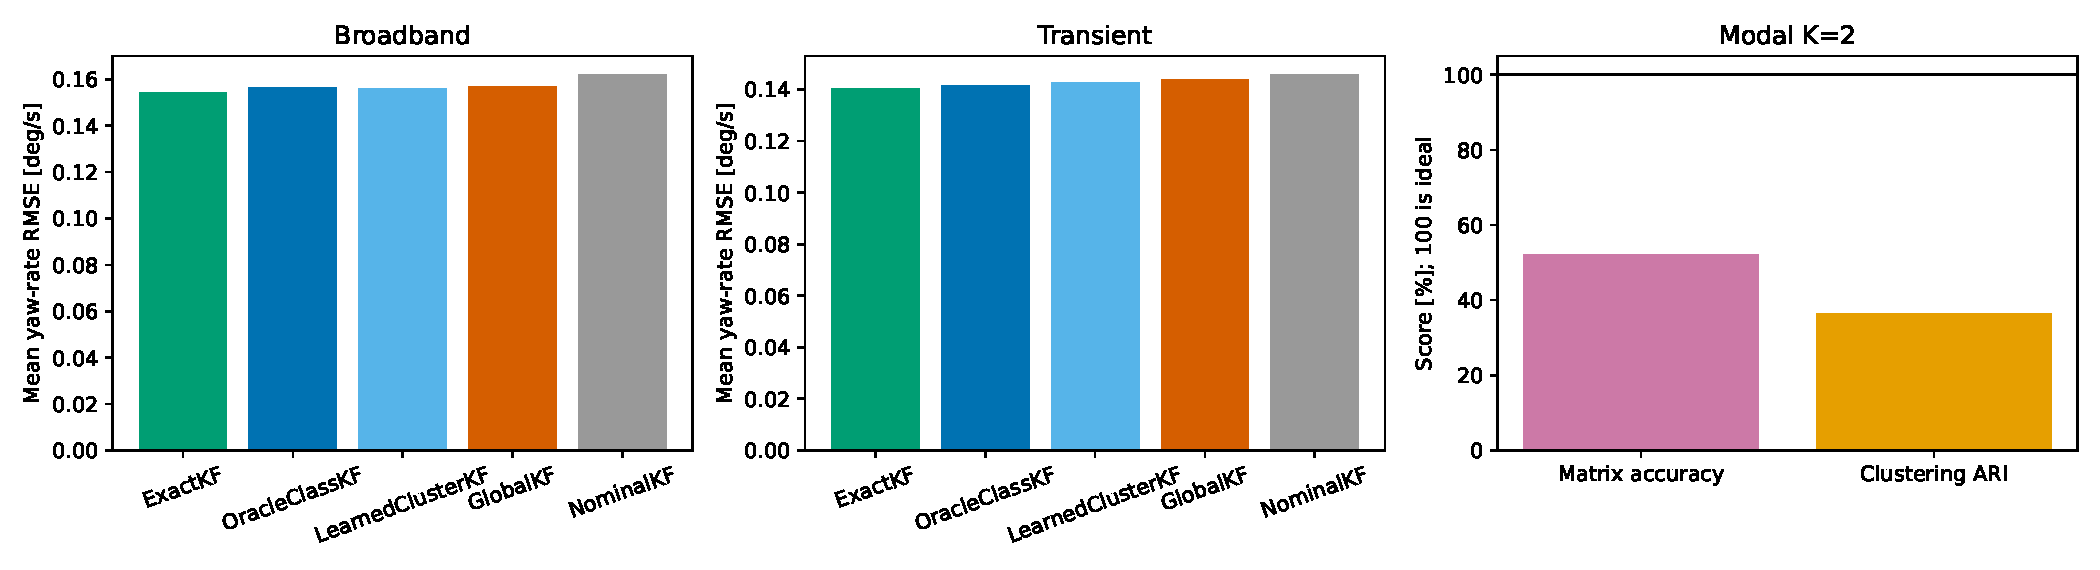
\includegraphics[width=0.98\linewidth]{../results/figures/experiment_10hd_measured_output_groups.pdf}
\caption{Development-only measured-output performance, local matrix accuracy,
and learned grouping quality in Experiment 10H-D.}
\label{fig:experiment10hd}
\end{figure}

\paragraph{Interpretation and decision.}
The positive 10H-C result does not survive the simplest end-to-end local
identification mechanism. This is an informative boundary: observability of
the five-state model does not imply that a mismatched nominal filter followed
by pseudo-state regression identifies physically comparable client updates.
Low pseudo-state prediction error can coexist with poor matrix accuracy and
poor clustering because all clients inherit the nominal observer's coordinate
and regularization bias.

The reserved confirmation fleets are not opened. Further progress requires a
joint state--parameter method that respects the fixed physical coordinates,
such as structured EM/prediction-error identification with the known
measurement map, or direct clustering of output innovations with a subsequent
groupwise model update. Simply reducing the ridge penalty or increasing the
number of mixture restarts would tune symptoms rather than resolve the
identification ambiguity. Privacy experiments are premature until this gate is
recovered.

\paragraph{Reproducibility.}
Configuration and implementation are in
\path{code/config/experiment_10hd.json} and
\path{code/experiments/experiment_10hd_measured_output_observer_groups.py}.
Development client records, candidate BIC scores, local-fit diagnostics,
paired comparisons, failed gate decisions, reserved confirmation seeds, and
provenance hashes are stored under \path{results}.
